\documentclass[12pt,letterpaper]{article}
\usepackage{fontspec}
\setmainfont{Times New Roman}
\usepackage{setspace}
\usepackage[utf8]{inputenc}
\usepackage[spanish, es-tabla]{babel}
\usepackage[version=3]{mhchem}
\usepackage[journal=jacs]{chemstyle}
\usepackage{amsmath}
\usepackage{amsfonts}
\usepackage{amssymb}
\usepackage{makeidx}
\usepackage{xcolor}
\usepackage[stable]{footmisc}
\usepackage[section]{placeins}
\usepackage{listings}
\usepackage[style=authoryear,backend=bibtex]{biblatex}
\addbibresource{ref1.bib}
\usepackage{tikz}
\usepackage{verbatim}
\usepackage{graphicx}
\usepackage{url}     
\usepackage{amsmath} 
\usepackage{tabularx}
\usepackage{ragged2e}
\usetikzlibrary{shapes.arrows}
\usepackage{siunitx}
\sisetup{mode=text, output-decimal-marker = {,}, per-mode = symbol, qualifier-mode = phrase, qualifier-phrase = { de }, list-units = brackets, range-units = brackets, range-phrase = --}
\DeclareSIUnit[number-unit-product = \;] \atmosphere{atm}
\DeclareSIUnit[number-unit-product = \;] \pound{lb}
\DeclareSIUnit[number-unit-product = \;] \inch{"}
\DeclareSIUnit[number-unit-product = \;] \foot{ft}
\DeclareSIUnit[number-unit-product = \;] \yard{yd}
\DeclareSIUnit[number-unit-product = \;] \mile{mi}
\DeclareSIUnit[number-unit-product = \;] \pint{pt}
\DeclareSIUnit[number-unit-product = \;] \quart{qt}
\DeclareSIUnit[number-unit-product = \;] \flounce{fl-oz}
\DeclareSIUnit[number-unit-product = \;] \ounce{oz}
\DeclareSIUnit[number-unit-product = \;] \degreeFahrenheit{\SIUnitSymbolDegree F}
\DeclareSIUnit[number-unit-product = \;] \degreeRankine{\SIUnitSymbolDegree R}
\DeclareSIUnit[number-unit-product = \;] \usgallon{galón}
\DeclareSIUnit[number-unit-product = \;] \uma{uma}
\DeclareSIUnit[number-unit-product = \;] \ppm{ppm}
\DeclareSIUnit[number-unit-product = \;] \eqg{eq-g}
\DeclareSIUnit[number-unit-product = \;] \normal{\eqg\per\liter\of{solución}}
\DeclareSIUnit[number-unit-product = \;] \molal{\mole\per\kilo\gram\of{solvente}}
\usepackage{cancel}
\usepackage{graphicx}
\usepackage{lmodern}
\usepackage{fancyhdr}
\usepackage[left=4cm,right=2cm,top=3cm,bottom=3cm]{geometry}


\usepackage{titlesec}
\usepackage{enumitem}
\titleformat*{\section}{\bfseries\large}
\titleformat*{\subsection}{\bfseries\normalsize}

%Creación del ambiente anexos
\usepackage{float}
\floatstyle{plaintop}
\newfloat{anexo}{thp}{anx}
\floatname{anexo}{Anexo}
\restylefloat{anexo}
\restylefloat{figure}

\usepackage[margin=10pt,labelfont=bf]{caption}

\usepackage{todonotes}

\usepackage[colorlinks=true, 
            linkcolor = blue,
            urlcolor  = blue,
            citecolor = black,
            anchorcolor = blue]{hyperref}
\usepackage{color}
\usepackage{multicol}

%======================================================================

\begin{document}
\onehalfspacing 
\thispagestyle{empty}
\begin{center}
\vspace{0.2cm}

\hrulefill

UNIVERSIDADE FEDERAL DE ALAGOAS\\
PRÓ-REITORIA DE PESQUISA E PÓS-GRADUAÇÃO\\
COORDENADORIA DE PESQUISA

\hrulefill

\vspace{0.5cm}

PROGRAMA INSTITUCIONAL DE BOLSAS DE INICIAÇÃO CIENTÍFICA\\PIBIC/UFAL/FAPEAL/CNPq

\vspace{1.0cm}

\textbf{\Large{RELATÓRIO PIBIC (2017 -- 2018)}}\\

\end{center}

\vspace{1.2cm}

\textbf{TÍTULO DO PROJETO DE PESQUISA:}

\underline{Análise de Sinais e Imagens com Distâncias Estocásticas e Diferenças de Entropias}

\textbf{TÍTULO DO PLANO DE TRABALHO:}

\underline{Desenvolvimento de Bibliotecas para Simulação e Inferência em Modelos para Imagens SAR}

\vspace{1cm}

\begin{table}[!h]
\begin{center}
\begin{tabularx}{\textwidth}{|X|X|X|}
\hline                              
\textbf{Nome Orientador/Unidade/Campus/Email} &  Alejandro César Frery Orgambide/Universidade Federal de Alagoas/Campus A.C. Simões/acfrery@gmail.com\\
\hline     
\textbf{Nome Bolsista ou Colaborador} & Marcos Gleysson Silva do Nascimento\\
\hline     
\textbf{Email/Fones} & mgsn@laccan.ufal.br/(82) 99671-0608\\
\hline     
\end{tabularx}
\end{center}
\end{table}

% Qual deles?
\begin{table}[!h]
\begin{center}
\begin{tabularx}{\textwidth}{|X|X|X|X|}
\hline                              
X & Bolsista CNPq &  &Bolsista FAPEAL\\
\hline             
& Bolsista UFAL &  &Colaborador\\
\hline             
& Bolsista PIBIC-Af&  &\\
\hline     
\end{tabularx}
\end{center}
\end{table}

\hrulefill   

%=================================================================

\newpage
\section*{\centering \textbf{RESUMO DO PROJETO}}
\hrulefill \\

\vspace{0.2cm}

A Teoria da Informação é um território interdisciplinar que perpassa a Probabilidade, a Estatística, e as Telecomunicações, e que tem produzido inúmeros resultados de relevância tanto teórica quanto do ponto de vista das aplicações. Algumas das ferramentas centrais da Teoria da Informação são as noções de entropia e de entropia relativa. A primeira mede a desordem de um sistema caracterizado por uma distribuição 
de probabilidade, enquanto a segunda mede quanto se perde ao descrever um processo utilizando uma distribuição de probabilidade que não é “a correta”. Esta última medida pode ser transformada em uma distância entre distribuições de probabilidade, e em uma estatística de teste. 

Ha duas frentes promissoras de pesquisa, dentre as inúmeras possibilidades que se abrem com a aplicação de ferramentas oriundas da Teoria da Informação. A primeira é voltada para a análise de séries temporais, e a segunda para imagens. Para ambas, é necessário definir um ou mais modelos possíveis, estimar as distribuições de interesse a partir dos dados disponíveis, e depois extrair atributos relevantes.

O trabalho de Gomez et al. (2015) mostra uma aplicação de distâncias entre distribuições na análise de imagens. Primeiramente, escolhem-se áreas da imagem que servem como protótipos das classes de interesse. Em cada passo de um método iterativo, cada pixel é atribuído a classe mais próxima, e essa distância é medida entre a distribuição do pixel a cada protótipo. Esta abordagem fornece resultados excelentes, mesmo em se tratando de dados notadamente difíceis de serem descritos e tratados com técnicas clássicas. 

Diversos desafios surgem na hora de tratar um problema com este tipo de técnicas. Há problemas analíticos ainda não resolvidos, que se constituem em uma linha de pesquisa avançada. Há também problemas de ordem computacional, mas que requerem por parte dos envolvidos um bom domínio das teorias que dão sustento as técnicas. É nesse terreno, o dos problemas computacionais que surgem na aplicação de ferramentas oriundas da 
Teoria de Informação a séries temporais e a imagens, que este trabalho se insere.


\textbf{Palavras-chave: Teoria da Informação; Imagens SAR; Séries Temporais} 


%=========================================================
%Modificar
\newpage
\section*{\centering \textbf{OBJETIVOS DO PROJETO DE PESQUISA}}
\hrulefill \\

\vspace{0.5cm}

O objetivo geral deste projeto é propor, desenvolver e avaliar ferramentas para facilitar o uso de técnicas avançadas de processamento e análise de imagens e sinais. Essas ferramentas são inovadoras, pois resultam de propostas recentes de pesquisas relacionadas a Teoria da Informação. 

Os objetivos específicos são produzir e testar duas ferramentas: ambiente gráfico para a análise não-paramétrica de séries temporais utilizando descritores de Teoria 
da Informação e bibliotecas de funções para simulação e estimação de parâmetros de modelos para imagens SAR.

Parte fundamental deste projeto é a verificação das propriedades numéricas do software desenvolvido. Estas propriedades são fundamentais para a aplicação dessas ferramentas na análise de dados. 


%=========================================================
%Modificar
\newpage
\section*{\centering \textbf{OBJETIVO ESPECÍFICO DO TRABALHO DO ALUNO}}
\hrulefill \\

\vspace{0.5cm}

Os objetivos específicos para esta frente de trabalho consistem em desenvolver técnicas de simulação e de estimação de parâmetros para distribuições de interesse na análise de imagens de radar de abertura sintética (Synthetic Aperture Radar - SAR). Essas distribuições seguem o modelo multiplicativo, e suas ocorrências podem ser obtidas por diversas maneiras. A estimação dos parâmetros dessas distribuições é, frequentemente, sujeita a instabilidades numéricas, viés e alta variabilidade. Por esse motivo, a literatura discute diversas técnicas para construir estimadores (por analogia, máxima verossimilhança, e com kernels), bem como para melhorá-los (com robustez, reamostragem e modificações analíticas).

Portanto, o objetivo deste trabalho consiste em Implementar uma biblioteca de
funções para a estimação de parâmetros de modelos para dados SAR, utilizando para esta implementação a plataforma R. 


%=========================================================

\newpage
\section*{\centering \textbf{ETAPAS DO PLANO DE TRABALHO}}
\hrulefill \\

\vspace{0.5cm}

O presente plano de trabalho tem por título Desenvolvimento de Bibliotecas para Simulação e Inferência em Modelos para imagens SAR.

As etapas necessárias para executar as metas com êxito e alcançar os objetivos propostos neste plano de trabalho são compostas por diversas atividades que vão desde a busca de materiais (artigos, livros, revistas, entre outros) relacionados à temática do projeto até a aplicação dos conhecimentos adquiridos na implementação de scripts utilizando a plataforma R. 

Para o início da pesquisa referente a minha frente de trabalho que tem por finalidade a implementação de uma biblioteca de funções para simulação e inferência em modelos de dados SAR foram buscadas uma série de boas referências para que fosse construída uma boa base de conhecimento para fornecer suporte às realizações dos objetivos finais do projeto.

Todo trabalho inicia-se com uma pergunta científica e foi solicitada ao orientador a pergunta referente ao meu plano de trabalho. A partir disso, diante da pergunta, foram buscados artigos e materiais de muita qualidade escritos por autores de alta relevância na temática.
O presente plano de trabalho envolve uma distribuição de probabilidade chamada de G-Intensidade Zero, dessa forma foram desenvolvidos estudos sobre essa distribuição para conhecer a fundo o seu comportamento e suas possíveis aplicações.

Após ter em mente a motivação que levou a GI0 a ser a distribuição foco da pesquisa, procurou-se analisar o funcionamento de geradores de números pseudoaleatórios sobretudo do gerador congruencial linear (do inglês, Linear congruential generator - LCG), obter uma maior familiaridade com a função densidade de probabilidade (f.d.p) da GI0 que indica a forma de como as variáveis aleatórias estão distribuídas e quais os parâmetros que envolvem tal distribuição, e além disso, investigou-se os diferentes métodos de geração de variáveis aleatórias GI0.

Nesse período de execução da pesquisa a utilização da plataforma R é bastante frequente, pois é onde estão implementadas as funções referentes a densidade e geração de variáveis GI0, e é através dessa plataforma que as demais funções estão sendo desenvolvidas. 


%=========================================================

\newpage
\section*{\centering \textbf{APRESENTAÇÃO E DISCUSSÃO DOS PRINCIPAIS RESULTADOS}}
\hrulefill \\

\vspace{0.5cm}

Como já explicado na seção anterior deste relatório, torna-se notável que foram obtidos avanços tanto do ponto de vista teórico quanto do ponto de vista prático.

Avanços teóricos ocorreram durante a pesquisa em virtude da busca de literatura referente às temáticas envolvidas no projeto, onde foram buscados diversos artigos de qualidade escritos por autores referência na temática em questão, bem como teses de dissertação de mestrado e doutorado de grandes pesquisadores que desenvolveram estudos envolvendo a área do presente projeto de pesquisa. Foram traçados alguns objetivos do ponto de vista prático nesse primeiro semestre da pesquisa os quais envolveram implementações na plataforma R e esses objetivos foram alcançados com êxito até o presente momento.

Diversas funções que se mostraram necessárias ao longo da execução do projeto foram implementadas no R, dentre elas a função de densidade de probabilidade da distribuição alvo dessa pesquisa, a GI0, bem como de outras distribuições como a Gama, Normal, Cauchy, Exponencial e a t, somado às implementações das funções foram desenvolvidos também os gráficos de densidade com pelo menos três valores diferentes para cada parâmetro da respectiva distribuição para fins de análise do comportamento da distribuição frente às alterações de parâmetro.

Além das funções de densidade, foi implementado também um gerador congruencial linear onde foram geradas algumas sequências de números pseudoaleatórios por meio desse gerador juntamente com a plotagem por histograma de cada sequência gerada. 

Por fim, dois métodos de geração de variáveis aleatórias GI0 foram definidos para serem implementados, o primeiro refere-se a geração de variáveis aleatórias GI0 pela razão de variáveis aleatórias Gama e o segundo a geração de variáveis aleatórias GI0 pelo Método da Inversão pela inversa da função de distribuição acumulada (f.d.a). A partir disso, pode-se perceber que existem diversos métodos de se gerar variáveis aleatórias de uma dada distribuição cada um com suas particularidades e neste projeto de pesquisa procura-se investigar diversas formas de se gerar variáveis aleatórias GI0 para definir critérios e avaliar a melhor forma de geração dessas variáveis.


%=========================================================

\newpage
\section*{\centering \textbf{CRONOGRAMA DE ATIVIDADES}}
\hrulefill \\

\vspace{0.5cm}

As atividades elaboradas para o respectivo plano de trabalho estão listadas logo abaixo:

\begin{small}
\begin{enumerate} 
  \item  Estudo dos conteúdos abordados no projeto por meio de artigos, livros, entre outros materiais
  \item  Estudo das funções a serem implementadas
  \item  Apresentação de seminário no LaCCAN para apresentar os avanços na literatura
  \item  Implementação das funções de densidade de distribuições de interesse e plotagem de gráficos
  \item Implementação da geração de variáveis aleatórias GI0 e de geradores congruenciais lineares
  \item  Implementação e validação numérica com dados simulados
  \item Analise da robustez dos algoritmos com dados simulados e reais 
  \item  Construção de exemplos de uso 
   \item  Otimização do código
   \item Validação, verificação e preparação de manuais e tutoriais de uso 

\end{enumerate}
\end{small}

\begin{figure}[!hbt]
	\begin{center}
    \vspace{-0.5cm}
		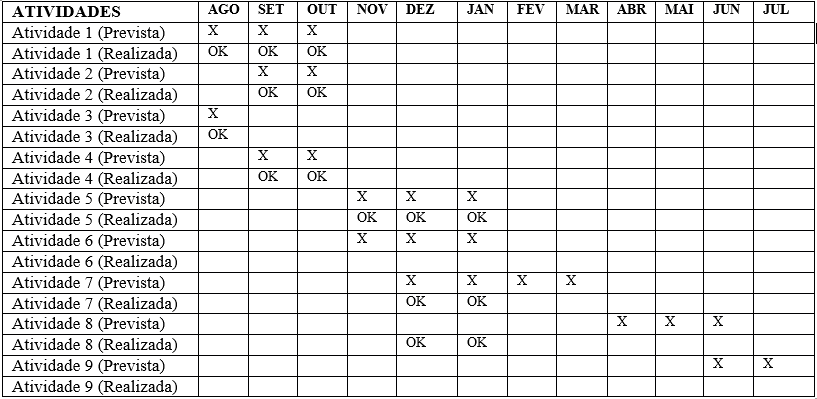
\includegraphics[width=0.9\columnwidth]{tabela-cronograma.png}
	\end{center}
\end{figure}

\newpage
Durante a execução do cronograma de atividades previsto, algumas atividades não foram concluídas como planejado por falta de tempo hábil para a conclusão da respectiva tarefa em virtude de alguns fatores que interferiram na execução do plano tais como o desafio de aliar as atividades de pesquisa com a demanda das disciplinas da graduação do pesquisador juntamente com o tempo que foi necessário para estudo de diversos tópicos da imensa área que permeia o presente projeto de pesquisa. Entretanto, mesmo com o cronograma apertado, os objetivos agora são executar as tarefas de forma mais eficiente e com agilidade de modo a permitir a conclusão de todas as atividades previstas no período estipulado para o projeto. Em virtude dos atrasos que houveram, também procurou-se adiantar algumas das atividades como, por exemplo, a parte de otimização de código onde procurou-se concomitantemente a implementação das funções otimizar o código que está sendo desenvolvido. 

%=========================================================

\newpage
\newpage
\section*{\centering \textbf{FATORES POSITIVOS E NEGATIVOS NA CONDUÇÃO DO PROJETO E PLANO DE TRABALHO}}
\hrulefill \\

\vspace{0.5cm}

Podemos citar como fatores positivos o fato de existir muitos materiais de qualidade (livros, artigos, entre outros) referentes ao tema do projeto da pesquisa, bem como o fato de existirem seminários semanalmente no Laboratório de Computação Científica e Análise Numérica (LaCCAN) que favorecem a aquisição de novos conhecimentos a respeito de diversos temas provenientes dos demais projetos de iniciação científica dos demais pesquisadores do laboratório. Além desses fatores positivos, podemos citar também o fato de existirem reuniões frequentes com o orientador onde podem ser mostrados os resultados obtidos, resolvidas algumas dúvidas e traçados os novos objetivos. 

Como fatores negativos podemos citar o fato de as disciplinas da graduação requisitarem um tempo grande o que acaba por sobrecarregar o pesquisador, além disso houve necessidade de um tempo consideravelmente grande para estudo dos assuntos que permeiam a área do projeto.  


%==============================================================================================================

\newpage
\section*{\centering \textbf{\LARGE{Referências bibliográficas}}}
\hrulefill \\

\nocite{*}

%\printbibliography%

GOMEZ, L. et al. Classification of complex Wishart matrices with a diffusion-reaction system guided by
stochastic distances. Philosophical Transactions of the Royal Society A: Mathematical, Physical and Engineering
Sciences, The Royal Society, v. 373, n. 2056, p. 20150118, Nov 2015. ISSN 1471-2962. 




\end{document}